\documentclass[10pt]{article}

\usepackage{fullpage}
\usepackage{graphicx}
\usepackage{mathtools}
\usepackage{setspace}
\usepackage{mdwlist}
\usepackage[center]{caption}
\onehalfspacing

\begin{document}
\title{Project Proposal\\Augmented Reality Image Processing System}
\author{Logan P. Williams \& Jos\'{e} E. Cruz Serrall\'{e}s}
\date{November 03, 2011}
\maketitle

\section{Abstract}
% should be revised, this is what we originally turned in 
In our project, we will implement an augmented reality system that can overlay a digital image on video of a real world environment. We begin by reading NTSC video from a video camera and storing it in ZBT SRAM. A picture frame with colored markers on the corners is held in front of the camera. We then perform chroma-based object recognition to locate the co-ordinates of the corners. Using these co-ordinates, we apply a low-pass filter (ArbiLPF) and a projective transformation (ArbiSkew) to project an image onto the dimensions of the picture frame. We then output VGA video of the original captured image, with the processed image overlayed on top of the frame. The overlayed image (the ``augmentation'') can be arbitrary. When this image is the frame of video that was previously displayed, we call the system ``recursive'', as we obtain the same image contained within itself.
\section{Top-Level Block Diagram}
\begin{figure}[h!]
\centering
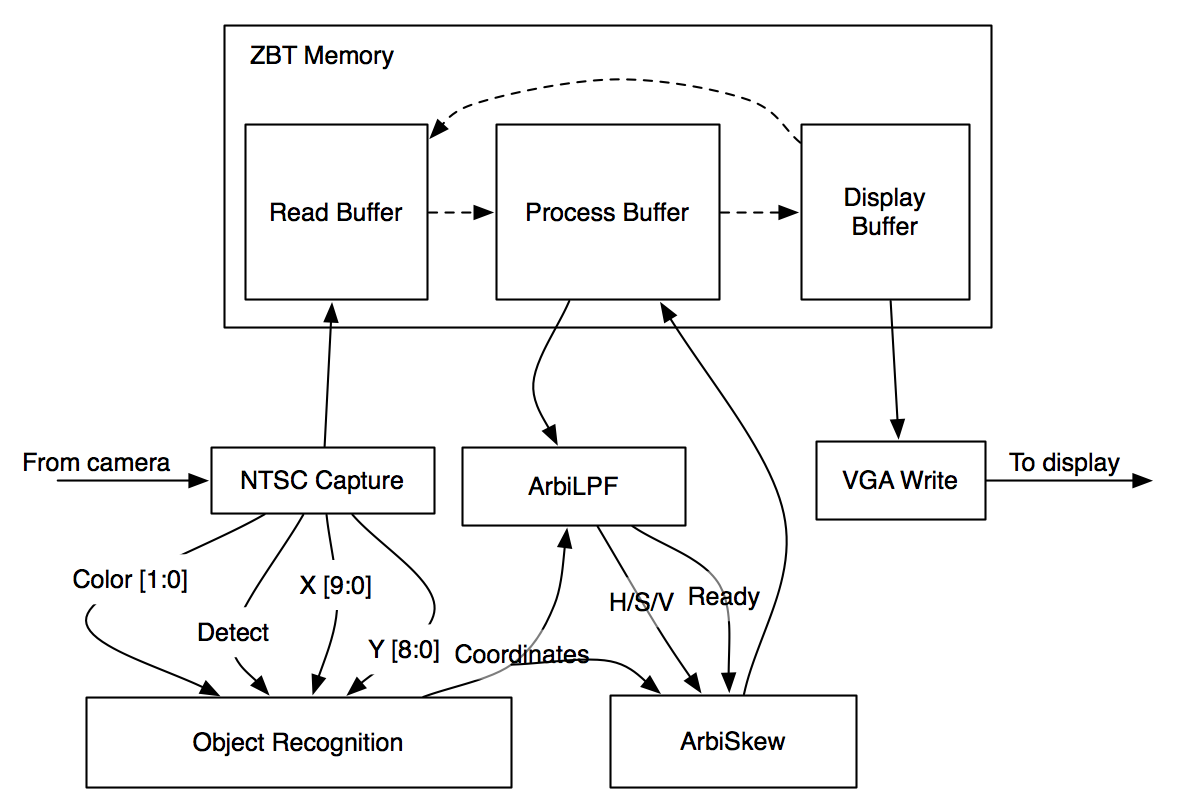
\includegraphics[width=0.62\textwidth]{block_diagram.png}
\caption{\emph{The block diagram of the augmented reality system.}}
\end{figure}
\section{Submodules}
% 1) inputs & outputs
% 2) some indication of its complexity and level of performance
%	a) number and type of arithmetic operations
%	b) size of internal memories
%	c) required throughput
%	etc.
% 3) how the module will be tested
% 4) who will be writing the module
\subsection{NTSC Capture (Logan)}
The NTSC capture module is almost unmodified from the code provided by 6.111. It takes as input an NTSC video signal, and writes pixels into ZBT Memory.

There are two modifications. The first allows the module to capture and store color data, converting it from Y/Cr/Cb to H/S/V. The second modification is added to support object recognition. When the Capture module sees a pixel of a hue that matches the target (blue, green, red, and yellow), it sends information (the color and its X/Y location) to the Object Recognition module. It also outputs a flag that goes high when the entire frame has been captured.

This module can be tested by connecting it to the VGA output module and ensuring that the video output is the image seen by the video camera.

\subsection{ZBT Memory (Jos\'{e})}
% Jose
The ZBT Memory module stores three 640x480 images in ZBT RAM. ZBT RAM was chosen instead of BRAM because the data in three 640x480 RGB images vastly exceeds our BRAM capacity. These three images will be (1) the image that is currently being captured, (2) the image that was just captured and to which skew will write its pixels, and (3) the image that is currently displayed. These three images will be henceforth referred to as ``capturing image'', ``processing image'', and ``displaying image'', respectively. The inputs to ZBT Memory are (1) the next pixel to be written to capturing image, (2) the next pixel to be written to processing image and (3) its index, (4) the index of the next pixel to be read from processing image, (5) the index of the next pixel to be read from displaying image as requested by the VGA Write module, and (6) the set of indices of the next set of pixels to be read from displaying image as requested by the ArbiLPF module. The outputs of ZBT Memory are (1) a pulse indicating whether a pixel was written to capturing image, (2) a pulse indicating whether a pixel was written to processing image, (3) the current pixel to be read from processing image, (4) a pulse indicating that this output was updated, (5) the current pixel to be read from displaying image as requested by the VGA Write module, (6) a pulse indicating that this output was updated, (7) the current set of pixels to be read from displaying image as requested by the ArbiLPF module, and (8) a pulse indicating that this output was updated.

The three images will be split between two ZBT RAM modules; as such, the ZBT Memory module will keep track of which image is in which block and intelligently return the correct pixel for each respective image given a relative index. Every NTSC capture refresh cycle (ie, every 1/30 seconds), the ZBT Memory module will switch the current processing image to be the new displaying image, the current displaying image to be the new capturing image, and the current capturing image to be the new processing image. Thus, reads and writes will be completely mandated by submodules and no data will have to be shifted around, improving efficiency.

The single write or read per cycle constraint that is imposed by each ZBT RAM module necessitates the use of a much higher clock speed than the standard 21.175MHz used for 640x480 at 60Hz output. Therefore, the clock speed will have to be at least approximately 120MHz for appropriate latency for this module. The ArbiLPF module, the ArbiSkew module, and the Object Recognition module should be run on the order of 90MHz, because this clock frequency allows for multiplications to be executed safely and allows the computationally intensive submodules enough time to complete all of their calculations.

The ZBT Memory will be a challenge to test thoroughly. The alternation of image locations will be tested with one testbench, and small sample images. Another testbench will be written to test the interface between the two RAM blocks and all of the read and write requests that they will be receive from the other submodules. Extensive care will be taken to ensure fairness among all of the submodules when contesting the memory, ie, not module should be favored too heavily among the other submodules. With a high enough clock frequency, this contention problem should not be a big issue.

\subsection{Object Recognition (Logan)}
The Object Recognition module collects ``interesting'' pixels located by the NTSC Capture module, and calculates the center of mass of each color, to find the location of the corners of the picture frame. It takes as input (1) the color of a detected pixel, (2) a flag that goes high for one clock cycle when a pixel is detected, (3) the X/Y coordinates of the pixel, and (4) a flag that goes high when the entire frame has been captured. It produces as output four sets of X/Y coordinates, one of the center of mass of each color.

The center of mass will be calculating with a simple linear weighting scheme, averaging the X and the Y coordinate for each pixel independently to find the center X/Y location, which are used by the ArbiLPF and the ArbiSkew module. This module can be tested with a simple test bench that provides some sample pixel locations, and tests to see if the module computes the center of mass correctly.

\subsection{ArbiLPF (Jos\'{e})}
% Jose
The inputs to ArbiLPF are (1) the downsampling coefficient (M), (2) the index of the pixel in displayed image to be filtered given this downsampling factor, (3) the set of pixels around the filtered pixels required for filtering, and (4) the pulse from the memory module. ArbiLPF applies a two-dimensional low-pass filter to this pixel by using surrounding pixels to calculate the convolution sum. The radial cutoff frequency of this 2D filter is of \( \frac{\pi}{M} \), in order to avoid aliasing in the ArbiSkew module. The outputs of ArbiLPF are (1) the pixel values of the output of the lowpassed version of this image, sampled at the given index, and (2) the indices of the set of pixels that are needed for filtering.

Based on the downsampling factor M, the filter will select a set of coefficients from a lookup table and convolve the image values with these coefficients. This table of coefficients will correspond to the coefficients of 2D extrapolations of 1D FIR Parks-McClellan filters with cutoff frequencies of \( \frac{\pi}{M} \). Due to the limited number of multipliers on the FPGA and the single-input, single-output of the RAM module, these 2D filters will be constrained to have at most 16 coefficients, which constrains the one-dimensional filters to have at most 4 coefficients. Due to these constraints, the ripple and transition width specifications of the 1D filters will have to be lax. The radial symmetry of these 2D filters will be exploited to reduce the number of required multiplications by a factor of 4, to at most 4 multiplications per color per pixel or 12 multiplications per pixel.

Due to the single-input, single-output nature of the RAM, the clock frequency of this module will have to be greater than 80MHz. Given relatively little contention from other blocks, ArbiLPF will elapse at least 9 cycles at 90MHz per pixel, yielding a latency of 0.03072 seconds or a little less than one NTSC refresh period. ArbiLPF will also have to perform roughly eight additions per cycle, but the timing constraints imposed by these additions are negligible when compared to the multiplications.

ArbiLPF will be tested by crafting a testbench module that accepts an arbitrary 640x480 image and outputs the output of the filter. Initially, an image with an impulse at the center will be used, which ideally should cause the filter to output the filter coefficients that are used. As basic functionality is tested, more complicated images will be used. Eventually, complex images will be processed both with the testbench and with MATLAB and will be compared using the 2D Fourier plots of these two outputs.

\subsection{ArbiSkew (Logan)}
% Logan
The inputs to ArbiSkew are (1) the hue, saturation, and value of the last pixel produced by ArbiLPF, (2) a ready signal held high for one clock signal when ArbiLPF has processed a new pixel, and (3) the four coordinates of the corners of the frame provided by the Object Recognition module.

This function maps the original rectangular image to any convex quadrilateral, provided that all sides of the destination quadrilateral are shorter than the original, which is inherent in the overall system. A graphic representation of the transformation is shown in Figure 2, on the next page.

\begin{figure}[h!]
\centering
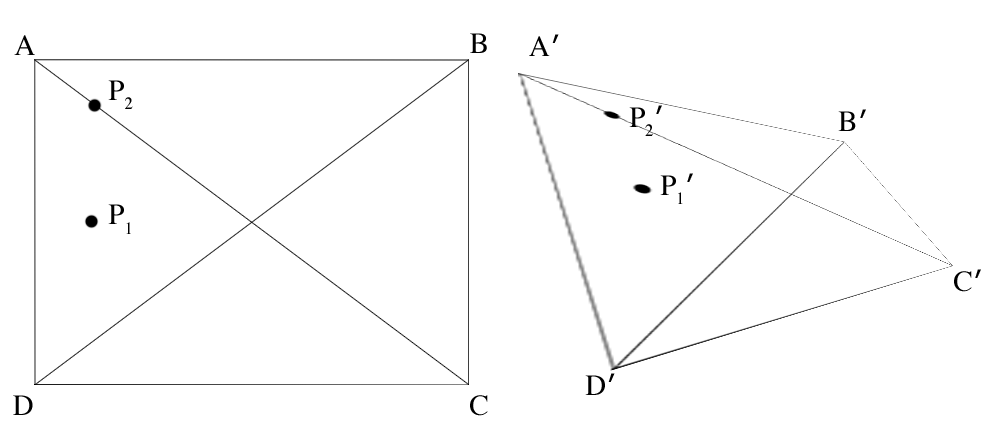
\includegraphics[width=0.65\textwidth]{arbiskew_graphic.png}
\caption{\emph{A visual representation of the result of the ArbiSkew module. Input is on the left, a possible output, for four coordinates $A\prime$, $B\prime$, $C\prime$, and $D\prime$ is on the right.}}
\end{figure}

Mathematically, the algorithm works as follows:
\begin{enumerate*}
\item Calculate the distance of line $\overline{A\prime D\prime}$ and assign it to $d_{ad}$.
\item Do the same for $\overline{B\prime C\prime}$ and assign it to $d_{bc}$.
\item Create two ``iterator points,'' point $I_A$ and $I_B$ initially located at $A\prime$ and $B\prime$.
\item Let $o_x = 0$ and $o_y = 0$
\item Calculate the distance between the iterator points, assign it to $d_i$.
\item Create a third iterator point, $I_C$ at the location $I_A$.
\item Assign the pixel value of $I_C$ to pixel $(o_x, o_y)$ in the original image.
\item Move $I_C$ along line $\overline{I_A I_B}$ by an amount $= \frac{d_i}{width_{original}}$.
\item Increment $o_x$.
\item Repeat steps 7--9 until $I_C = I_B$.
\item Move $I_A$ along line $\overline{A\prime D\prime}$ by an amount $= \frac{d_{ad}}{height_{original}}$.
\item Move $I_B$ along line $\overline{B\prime C\prime}$ by an amount $= \frac{d_{bc}}{height_{original}}$.
\item Increment $o_y$.
\item Repeat steps 5--13 until $I_A = D\prime$ and $I_B = C\prime$.
\end{enumerate*}

This is feasible on the FPGA by using lookup tables to calculate $\sin$, $\cos$, and $\arctan$ for angle calculations. Besides that, it needs a relatively small number of multiplications, just two per pixel in the original image, and four per line in the original image. There is also a square root that is needed once per line, this can be implemented with either a look up table, or by using an iterative method of calculation.

The ArbiSkew module can be tested by creating a test bench that provides a series of test pixels as input. The output generated in ModelSim by ArbiSkew can then be compared with the output generated by a MATLAB implementation of ArbiSkew.

\subsection{VGA Write (Jos\'{e})}
% Jose
The VGA Write section is straightforward and will basically be a clone of the VGA code used in Lab 2 (Pong). Essentially, the output will be refreshed at a rate of 60Hz and output at a resolution of 640x480 pixels. This module will read the pixel values from displayed image and assign it based on the hcount and vcount variables, which will be incremented accordingly. This module will be tested by loading a standardized image to memory and verifying whether VGA Write displays this image properly on the monitor.

\section{External Components}
We will be using two standard external components: an video camera that provides NTSC composite video out, to be provided by the 6.111 staff, and a VGA display.

\section{Project Deadlines}
% A calendar-like view of what deadlines we'll set ourselves, when everything should be operational, etc. Maybe this could be collapsed into the submodules section
\begin{itemize}
\item 11-11-2011 - Finalized Block Diagram
\item 11-18-2011 - First draft of ArbiLPF, ArbiSkew, and ZBT Memory written
\item 11-24-2011 - VGA Write and NTSC Capture first drafts written; ArbiLPF, ArbiSKEW, ZBT Memory fully tested
\item 12-01-2011 - NTSC Capture and VGA Write fully tested; start of full integration
\item 12-08-2011 - Full integration
\end{itemize}

\end{document}
